\chapter{Teil von Roland Gisler}

\section{Architektur}

\section{Testing}

\subsection{Ziele für gute Tests}

Durch das Erstellen von Testcode wird die Softwarequalität nachweislich gesteigert. Damit bei Regresstests Zeit gespart werden kann sollte die Testausführung so weit als möglich automatisiert werden. Die Testfälle sollten möglichst früh im Projekt mithilfe der Use Cases erstellt werden. Zudem sollte man die Testfälle möglichst kurz und einfach halten. Dadurch werden die Testfälle stabiler gegen Veränderungen und defekte lassen sich schneller lokalisieren. Als Basis sollten die normalen Abläufe getestet werden aber auch absichtlich provozierte Fehler und nicht erlaubte Vorgänge sollen ebenfalls getestet werden. Folgendes Ziel sollte immer vor Augen gehalten werden:
\begin{quote}
Testfälle gerade so komplex wie nötig, und so einfach wie möglich halten!
\end{quote}

\subsection{Testarten}

Neben der Unterteilung in Unit-, Integrations- und Systemtests, können Tests auch in folgende Kategorien aufgeteilt werden:
\begin{description}
	\item[Funktionale Tests:] Bei dieser Testart wird die gesamte Applikation aus der Sicht des Endbenutzers getestet. Es wird die Business- und die Applikationslogik getestet. Diese Testart ist sehr aufwendig und sollte wenn möglich automatisiert werden. 
	\item[Performance-/Stresstests:] Auf der einen Seite wird ein klassisches Profiling (Memorybedarf, Antwortzeit) durchgeführt. Es wird jedoch auch getestet wie die Anwendung bei hoher Belastung durch viele Clients reagiert (Queueing oder Zurückweisen von Anfragen).
	\item[Sicherheitstests:] Die Testart testet eine Applikation auf verschiedene Sicherheitslücken. Diese Testart ist vor allem bei Webapplikationen wichtig, um z.B. SQL-Injection zu verhindern.   
\end{description}

\subsection{Testdoubles}

Bei einer Schichten-Architektur welche Bottom-Up entwickelt wurde, besteht die Gefahr dass bei Unit-Tests alle unteren Schichten mit getestet werden. Dadurch steigt die Ausführungszeit und die Abhängigkeiten. Diese Tests sind in diesem Fall Integrationstests und nicht mehr Unit-Tests.
Um die Schichten voneinander zu entkoppeln werden Testdoubles eingesetzt. Um Testdoubles erfolgreich einzusetzen, muss ein entsprechend gutes Design nach SOLID vorliegen. Vor allem das Dependency Inversion Principle (DIP) sollte beachtet werden. Abbildung \ref{fig:test-doubles} zeigt eine Übersicht über alle Testdoubles.
\begin{figure}
\centering
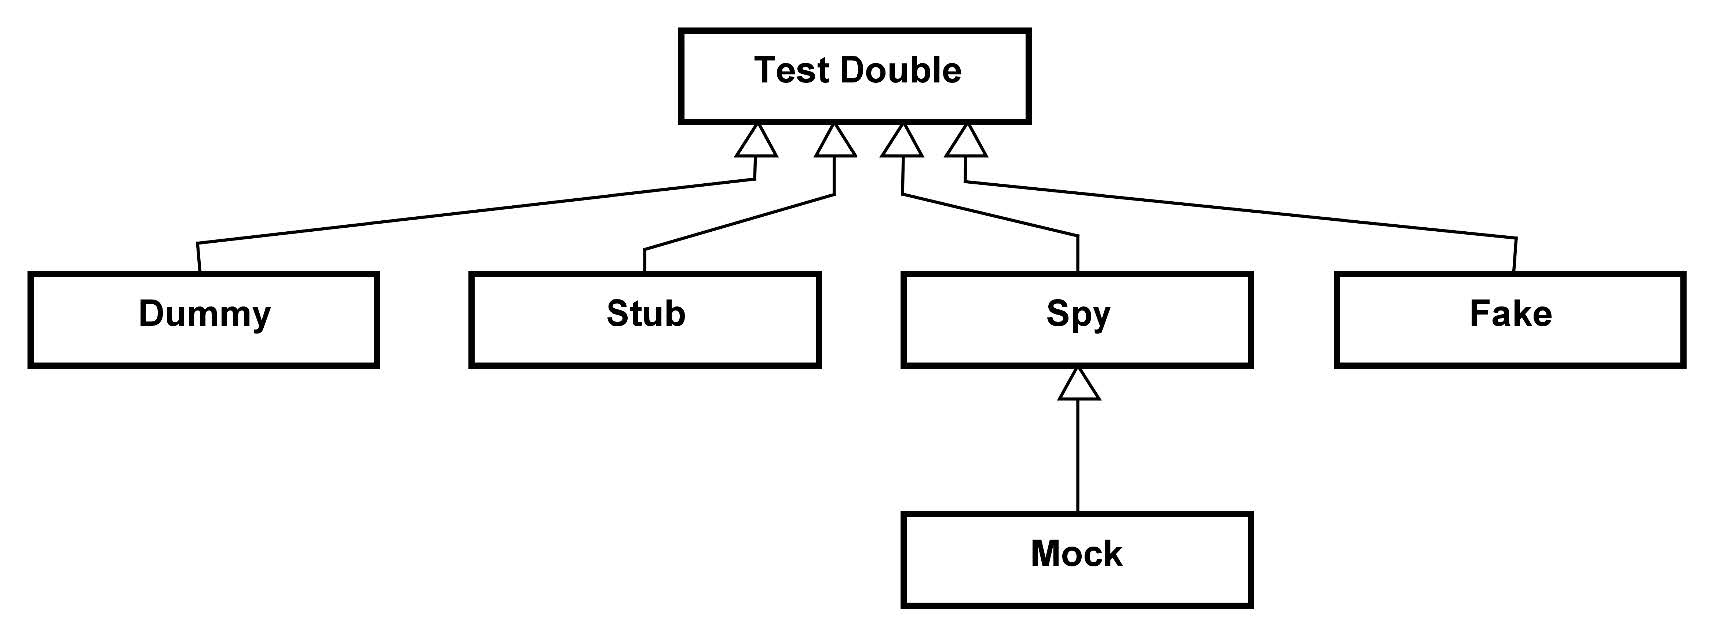
\includegraphics[width=0.7\linewidth]{fig/test-doubles}
\caption{Übersicht Test Doubles}
\label{fig:test-doubles}
\end{figure}
Nachfolgend werden alle Test Doubles im Detail beschrieben:
\begin{description}
	\item[Dummy:] Ein Dummy ist eine primitive (häufig leere) Ersatz-Implementation, welche als Parameter an eine Methode übergeben wird. Der Parameter muss für den Test vorhanden sein aber dessen Nutzung ist nicht relevant. Häufig geben Dummys einfach \texttt{null} zurück.
	\item[Stub:] Ein Stub liefert einen sinnvollen, vordefinierten Wert zurück. Für verschiedenen Testziele werden unterschiedliche Stub-Implementationen (z.B. für Fehlerfall) verwendet.
	\item[Spy:] Ein Spy liefert dynamisch Werte zurück und merkt sich die Methoden welche an ihm aufgerufen werden. Das erlaubt ein ''Behavior''-Testing.
	\item[Mock:] Ein Mock macht das gleiche wie der Spy, jedoch verifiziert er gleich selbst ob eine Methode aufgerufen wurde. Mocks werden typischerweise zur Laufzeit von Frameworks mit dem \emph{Proxy-Pattern} erstellt.
	\item[Fake:] Alternative Implementation, welche eine Komponente mit vernünftigem Aufwand ersetzen kann. Ein Fake ist manchmal besser als die eigentliche Implementation aber sehr aufwendig zu entwickeln.
\end{description}
Dummy und Stubs werden eingesetzt wenn man mit wenig Aufwand eine bessere Testisolation erreichen will. Die Test werden dadurch robuster. Spys und Mocks sind die Universalwaffen, werden jedoch oft zu häufig eingesetzt. Mit Mocks sollte man sparsam umgehen, weil sich sonst der Testcode zu stark an den Implementationscode koppelt. Ein Fake ist sehr aufwendig zum Entwickeln und wird praktisch nie eingesetzt.

\subsection{Testen von DB-Applikationen}

Die Herausforderung beim Testen von DB-Applikationen ist die Datenmanipulation durch die Testfälle. Damit diese Manipulationen reproduzierbar bleiben, muss der Datenbankinhalt vor und nach dem Test definiert/verifiziert werden. Um dies zu erreichen muss ein Testdatenmanagement betrieben werden. Beim Testdatenmanagement werden Testdaten pro Testfall bereitgestellt und aktiv gewartet.
Für das Testen von DB-Applikationen gibt es verschiedene Ansätze:
\begin{itemize}
	\item Initialisierung und Verifikation von Testdaten mit Frameworks (z.B. DBUnit)
	\item Verwendung von mehreren DB-Instanzen auf nur einem Server (z.B. 1 für Entwickler und 1 für Buildserver). Schwierig Schemas synchron zu halten und evtl. Konflikte bei paralleler Ausführung.
	\item Lokale Datenbank pro Entwickler, Buildserver usw. Je nachdem nicht möglich wegen Lizenzen jedoch keine Konflikte bei paralleler Ausführung.
	\item Nach den Tests ein Transaction Rollback durchführen (im Tear Down)
	\item In-Memory-Datenbank für jeden Test (langsam weil DB jedesmal aufgebaut werden muss)
\end{itemize}

\subsection{Testen von GUI-Applikationen}

Bei GUI-Applikationen stellt die GUI selber die Schnittstelle bereit. Die Interaktion mit der GUI muss demnach simuliert werden um Tests automatisiert durchführen zu können. Auch die Verifikation der Testergebnisse muss optisch erfolgen. Für das Testen von GUI-Applikationen werden zwei Ansätze verfolgt:
\begin{description}
	\item[Record \& Play:] Ein manueller Test wird aufgezeichnet, abgespielt und danach überprüft. Dies ist nicht zu empfehlen, weil die Prüfung schwierig/unsicher ist.
	\item[Frameworks:] Das GUI-Framework wird um die Testbarkeit erweitert. Diese Test müssen aufwendig programmiert werden. Es entsteht so eine starke Kopplung an die interne GUI-Struktur und man testet nie das Endresultat. Beispiele für GUI-Frameworks sind UISpec4J (Swing) oder TestFX (JavaFx).
\end{description}

\subsection{Testen von Web-Applikationen}

Web-Applikationen lassen sich aufgrund ihres strikten Request-/Response-Modell sehr gut testen, weil auf jede Anfrage eine definierte Antwort kommen muss. Stress- und Securitytests lassen sich so ebenfalls einfach automatisieren. In der Praxis wird diese Möglichkeit oft zu wenig genutzt. Es existieren aber für Java einige Frameworks:
\begin{itemize}
	\item HttpUnit
	\item HTMLUnit
	\item JWebUnit
	\item Selenium
\end{itemize}
Eine Voraussetzung für die Verwendung dieser Frameworks ist ein sauberer HTML-Code (z.B. alle Elemente mit id versehen). Diese Frameworks simulieren Browserzugriffe und analysieren die Antwort vom Server.
 
Web-Applikationen mit Web 2.0 Technologien (HTML 5, Ajax, JavaScript) sind schwieriger zu Testen. Diese Applikationen werden mit echten Browsern mit einem Test-Plugin getestet. Die Grundlage ist die Browser-Automation, wobei SeleniumHQ und Arquillian zwei Frameworks sind die das unterstützen. 

\section{SOLID}

Das SOLID-Prinzip fasst fünf wichtige Designprinzipen zusammen:
\begin{itemize}
	\item Single Responsibility Principle
	\item Open Closed Principle
	\item Liskov Substitution Principle
	\item Interface Segregation Principle
	\item Dependency Inversion Principle
\end{itemize}
Durch die Einhaltung der SOLID-Prinzipien erreicht man ein besseres Design. Besseres Design heisst konkret:
\begin{itemize}
	\item höhere Wiederverwendbarkeit
	\item leichtere Verständlichkeit / Lesbarkeit
	\item (stark) verbesserte Testbarkeit
	\item vereinfachte Wartung
	\item verbesserte Erweiterbarkeit
	\item leichteres Refactoring
\end{itemize}

\newpage

\subsection{Single Responsibility Principle}

\begin{itemize}
	\item Unix-Philosophie: «Tu nur ein Ding, genau ein Ding, das aber richtig!»
	\item Eine Klasse hat möglichst nur \textbf{eine} Zuständigkeit (siehe Listing \ref{lst:srp-interface})
	\item Eine Klasse hat somit nur \textbf{einen} Grund zur Änderung
	\item Änderungen oder Erweiterungen sollten sich auf möglichst wenige Klassen beschränken (hohe Kohäsion bleibt erhalten).
	\item Viele kleine Klassen sind besser als wenige grosse Klassen
	\item Wichtiger Nebeneffekt: Stark verbesserte Testbarkeit!
\end{itemize}

\begin{lstlisting}[caption={Schlechtes Interface nach SRP},label=lst:srp-interface]
// Zwei Aufgaben: Verbindungsaufbau und Datenübertragung
interface Modem {
	public void dial(String phoneNumber);
	public void hangup();
	public void send(char c);
	public char receive();
}
// Besser zwei Interfaces
interface Connection {
	public void dial(String phoneNumber);
	public void hangup();
}
interface Transmit {
	public void send(char c);
	public char receive();
}
\end{lstlisting}

\subsection{Open Closed Principle}

\begin{itemize}
	\item Eine Software-Entität soll offen für Erweiterungen, aber geschlossen gegenüber Modifikationen sein
	\item Mit OCP senkt man das Risiko neue Fehler einzubauen, weil man bestehenden Code nicht ändern muss
	\item Häufig über Einsatz des Strategy-Patterns (GoF) erreicht (siehe Listing \ref{lst:ocp-strategy})
\end{itemize}

\begin{lstlisting}[caption={Strategy Pattern um OCP umzusetzen},label=lst:ocp-strategy]
// Was passiert, wenn eine (oder hundert) neue Operation ergänzt werden soll?
double calc(Operation op, double arg1, double arg2) {
	double result = 0.0;
	switch (op) {
		case Addition:
			result = arg1 + arg2; break;
		case Subtraktion:
			result = arg1 - arg2; break;
		default:
			throw new IllegalArgumentException(); break;
	}
	return result;
}
// Pro neue Operation wird eine Klasse erstellt, welche das Interface Operation implementiert
interface Operation {
	double calc(double arg1, double arg2);
}
double calc(Operation op, double arg1, double arg2) {
	return op.calc(arg1, arg2);
}
\end{lstlisting}

\subsection{Liskov Substitution Principle}

\begin{itemize}
	\item Gut über den Sinn/die Korrektheit von Spezialisierungen nachdenken:
	\begin{itemize}
		\item Subtypen sollten sich so verhalten wie ihre Basistypen
		\item Meist ist Komposition der Vererbung vorzuziehen!
	\end{itemize}
	\item Verifiziere Entscheide mit folgenden Sätzen:
	 \begin{itemize}
		\item Subtyp ist ein (is-a) Basistyp (Vererbung)
		\item Subtyp verhält sich (behaves-as) wie ein Basistyp (Komposition)
	 \end{itemize}
	\item Macht die Implementation von \texttt{equals()} Schwierigkeiten, sollte man unbedingt die Vererbung hinterfragen!
	\item Tipp: Vererbung konsequent verhindern (\texttt{final}): Nur dort wo sinnvoll und vorgesehen explizites Design für Spezialisierungen (Design for inheritance or else prohibit it).
\end{itemize}

\subsection{Interface Segregation Principle}

\begin{itemize}
	\item Schnittstelle strikt von Details der Implementation trennen (Ist mit Java einfach: Wir haben Interfaces!)
	\item Schnittstellen sollen eine hohe Kohäsion haben
	\item Basisklassen sollten nichts von ihren Spezialisierungen wissen
	\item Kopplung zwischen Komponenten soll minimal sein
	\item Viele kleine (schmale) Schnittstellen sind besser als eine zu grosse (fette) Schnittstelle
	\item Population von Schnittstellen vermeiden (möglichst keine Vererbung von Schnittstellen)
\end{itemize}

\subsection{Dependency Inversion Principle}

\begin{itemize}
	\item DIP ist nicht gleich Dependency Injection!
	\item High-Level Klassen sollen nicht von Low-Level Klassen abhängig sein, sondern beide von Interfaces (siehe Abbildung \ref{fig:dip-beispiel})
	\item Interfaces sollen nicht von Details abhängig sein, sondern Details von Interfaces
	\item Isolation von Klassen vereinfacht/ermöglicht die Testbarkeit (ggf. auch mit Einsatz von Test Doubles)
	\item Auflösung von Dependencies über Dependency Injection (DI)
\end{itemize}

\begin{figure}[h!]
	\centering
	\begin{subfigure}[b]{0.8\textwidth}
		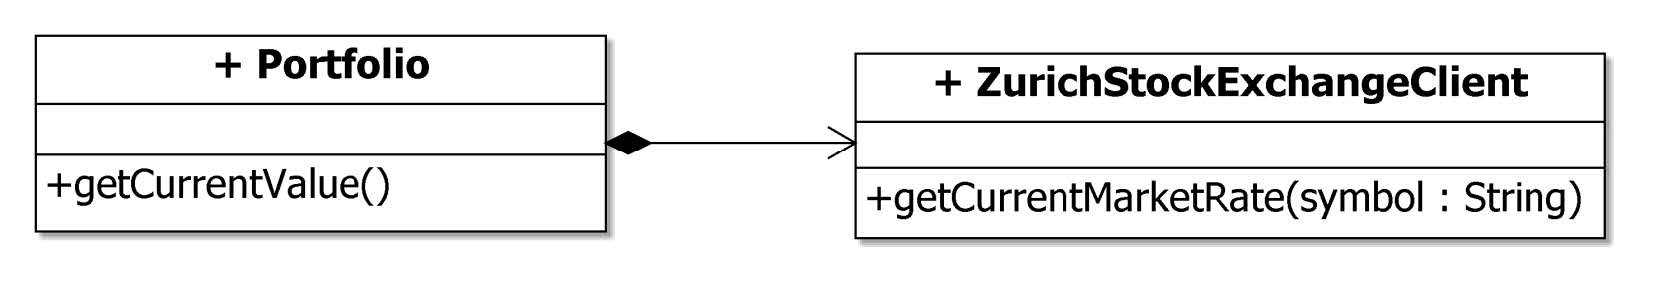
\includegraphics[width=\textwidth]{fig/dip-schlecht}
		\caption{High-Level-Klasse \texttt{Portfolio} ist abhängig von Low-Level-Klasse \texttt{ZurichStockExchangeClient} $\rightarrow$ Schlecht!}
	\end{subfigure}
	\begin{subfigure}[b]{\textwidth}
		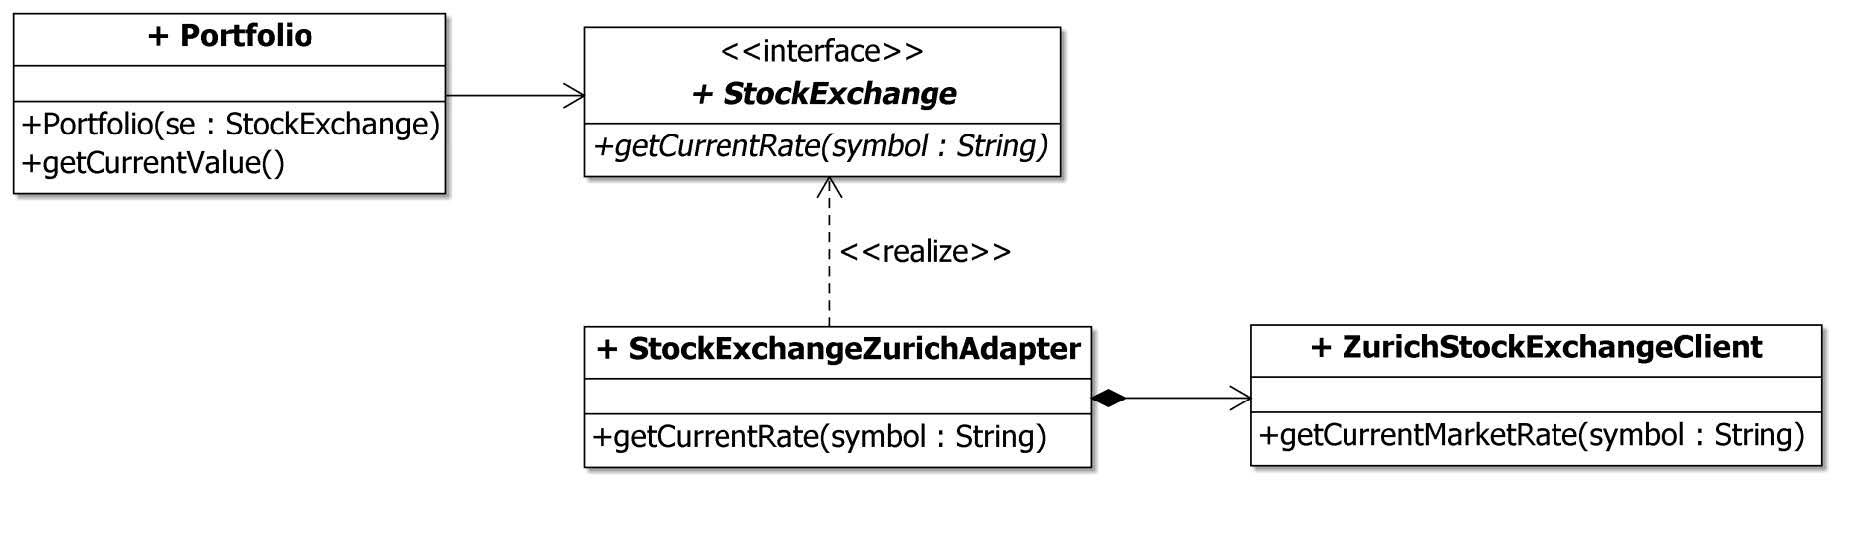
\includegraphics[width=\textwidth]{fig/dip-besser}
		\caption{Bessere Lösung: \texttt{Portfolio} unabhängig von Implementationsdetails}
	\end{subfigure}
	\caption{Beispiel DIP}\label{fig:dip-beispiel}
\end{figure}
